\chapter{Discussion}

\section{Consistency in Game Experience}


Figure~\ref{fig:US_Consistent_Speaking} shows the eSFQ game experience ratings for players with and without common languages, when communicating only by speaking. The experience ratings by the two player groups varied significantly. However, as shown in Figure~\ref{fig:US_Consistent_Bodylanguage}, the ratings between players with and without common languages was much more consistent when communicating via only body language. The average absolute difference in ratings was 22.4\% across the 8 indexes when communicating by speaking, compared to 6.25\% by body language only.

\begin{figure}[!h]
\centering
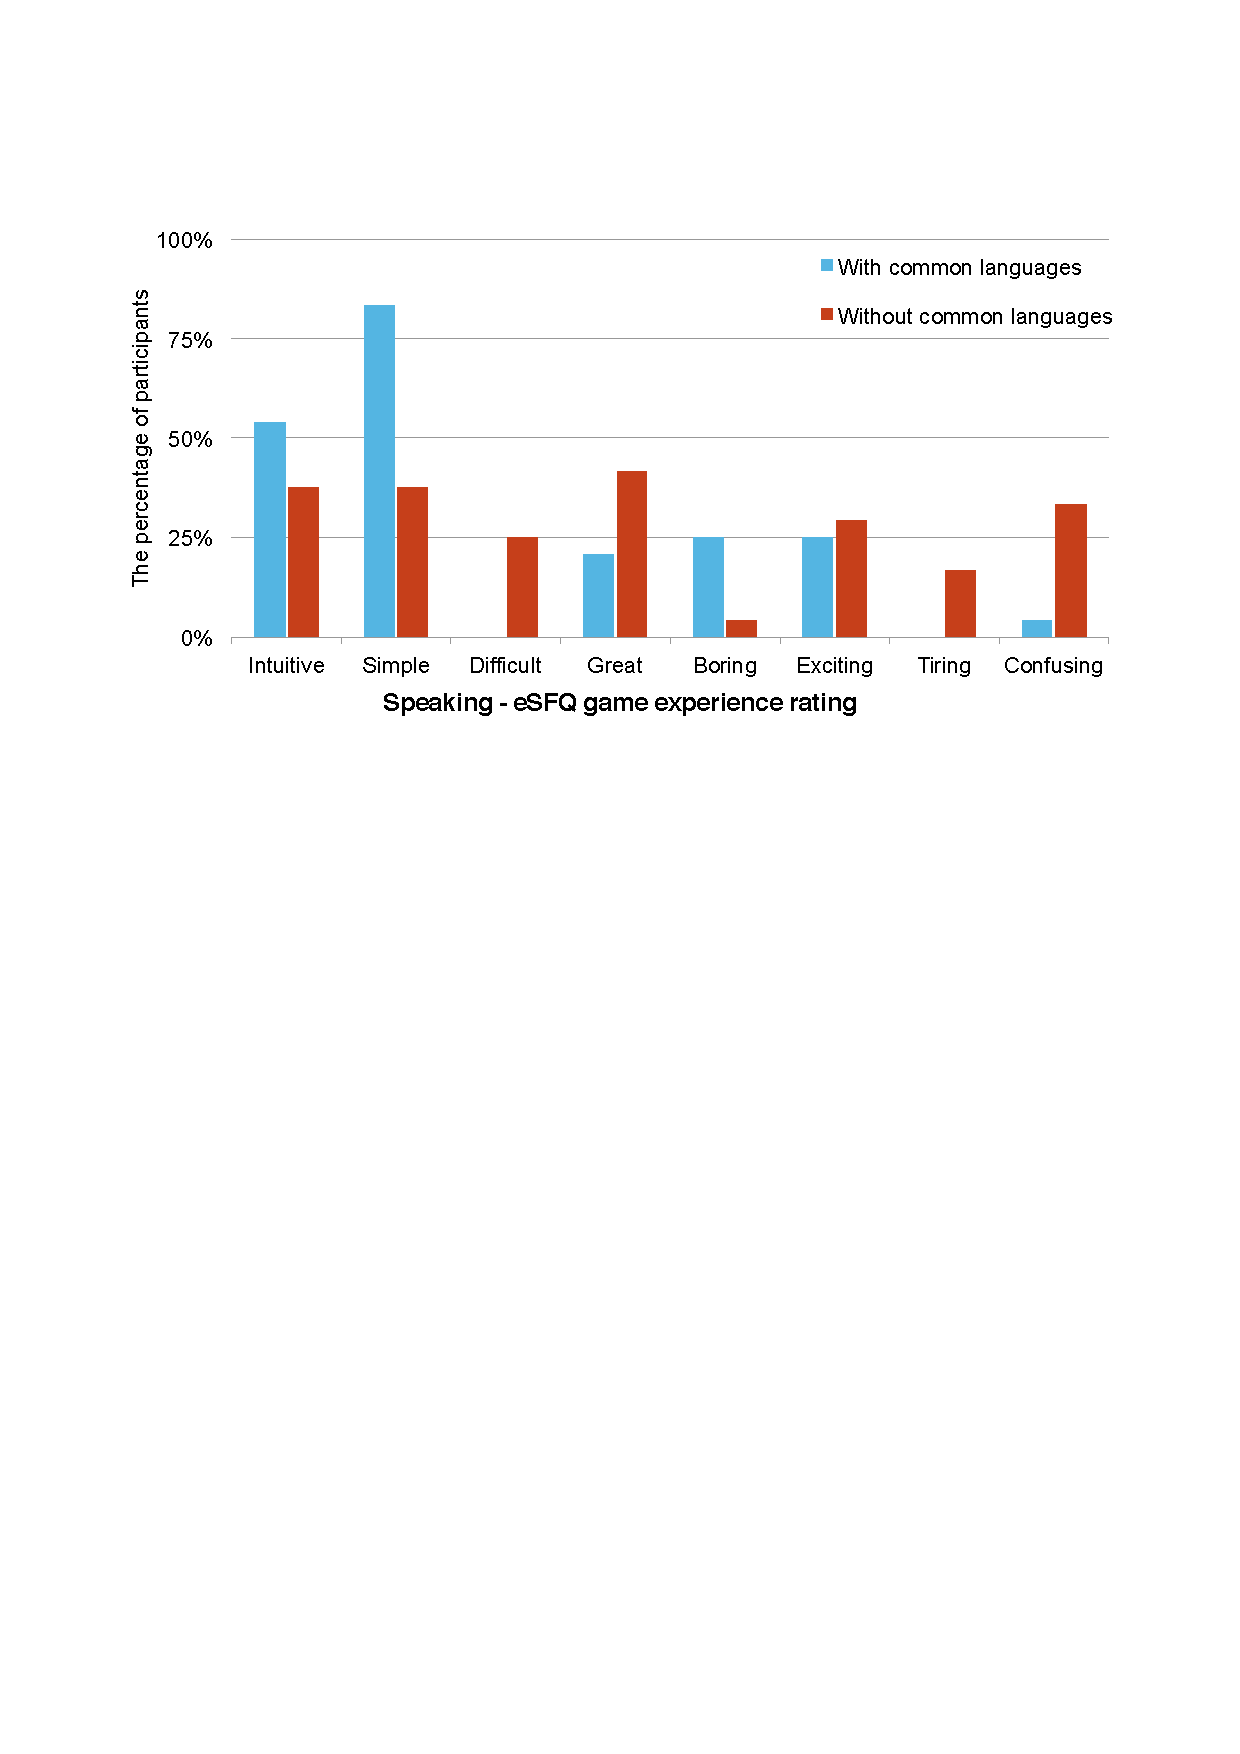
\includegraphics[width=1.0\columnwidth]{Figures/US_Consistent_Speaking.pdf}
\caption{Index patterns of eSFQ game experience rating for speaking}
\label{fig:US_Consistent_Speaking}
\end{figure}

\begin{figure}[!h]
\centering
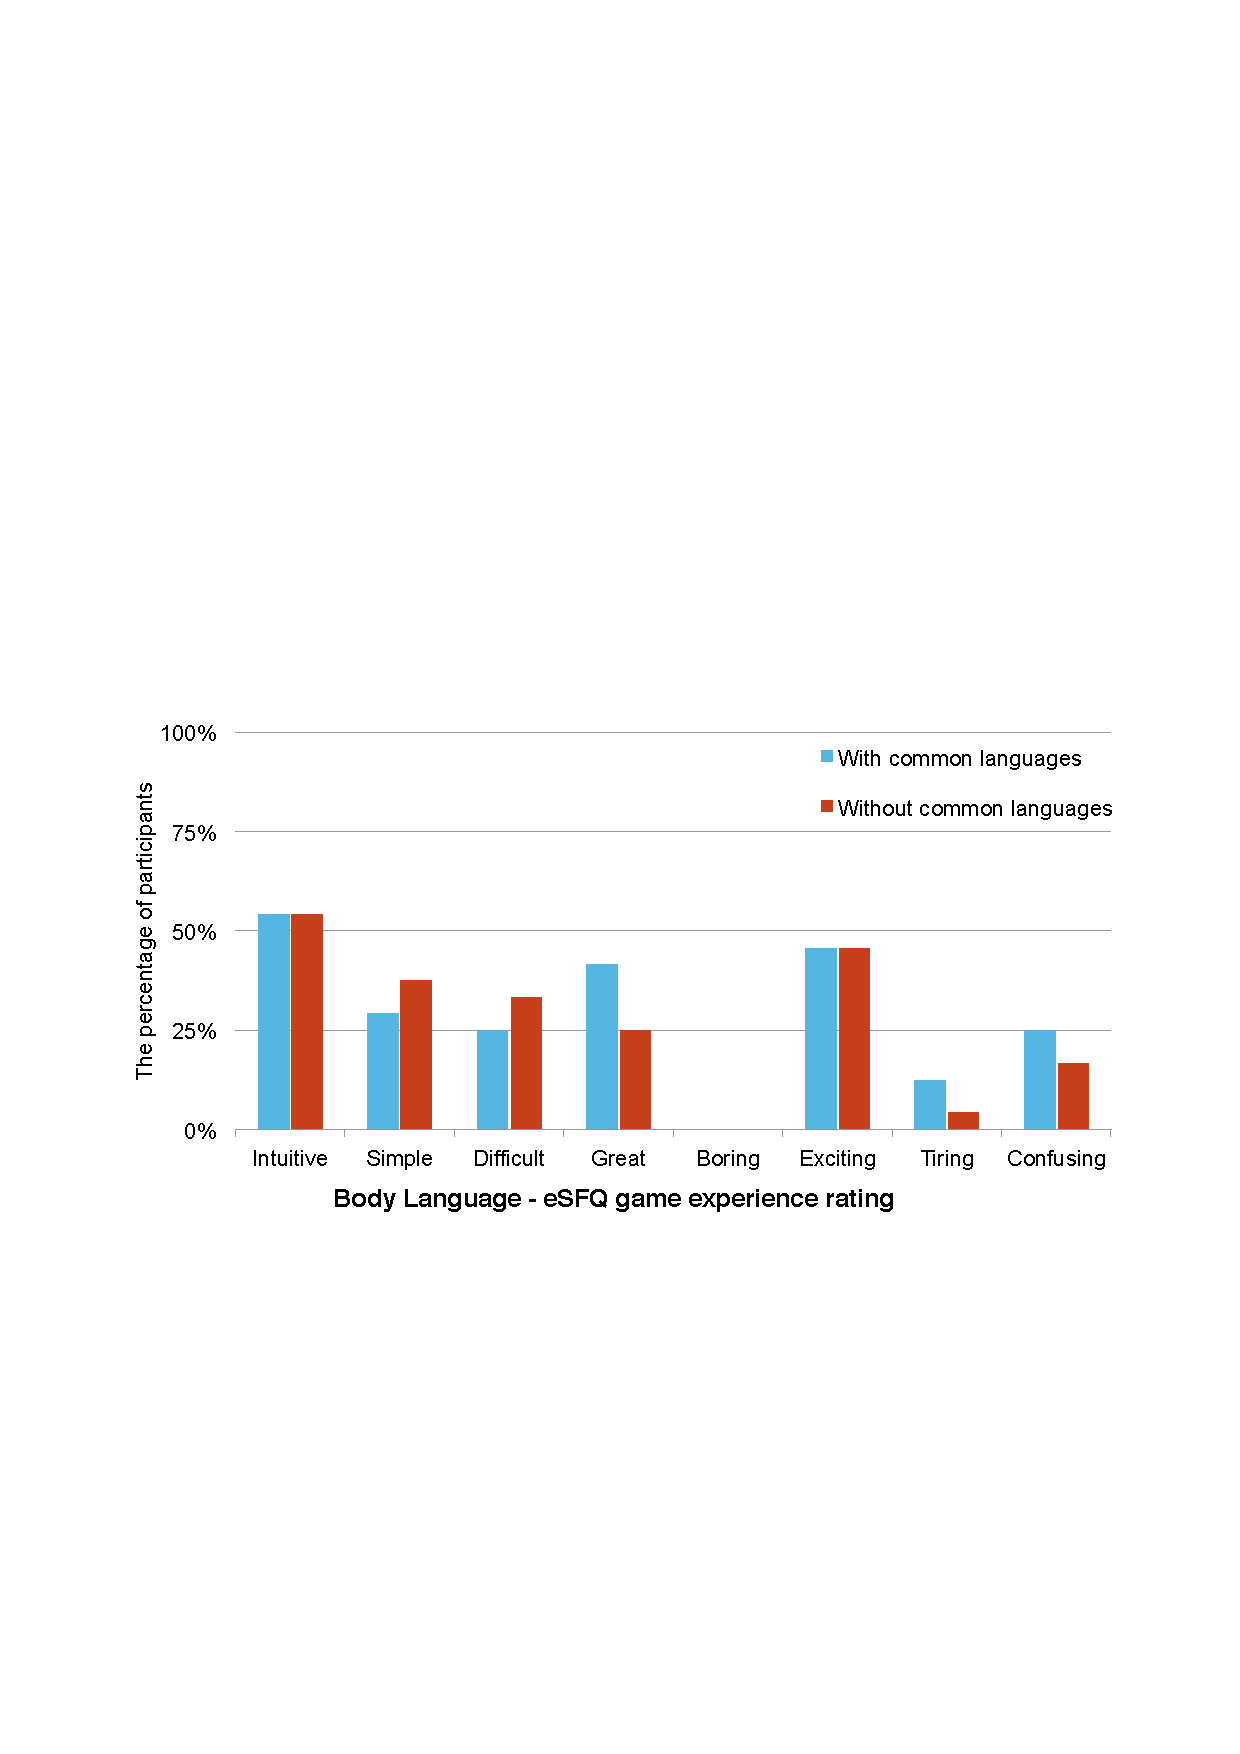
\includegraphics[width=1.0\columnwidth]{Figures/US_Consistent_Bodylanguage.pdf}
\caption{Index patterns of eSFQ game experience rating for body language}
\label{fig:US_Consistent_Bodylanguage}
\end{figure}



\section{Communication Patterns}
We summarize the communication patterns we observed when participants were communicated by: speaking, body language, and both speaking and body language.

\subsection{Speaking}
For participants with common languages, communicating by speaking was straight-forward. For participants without common languages, although there were language barriers, they still found ways communicate with each other by tones, short words, and sounds.

\begin{enumerate}
   \item Simple words: participants spoke simple words and short sentences. For example, Japanese speakers would say ``hai (yes)'', ``ie (no)'', ``koko (here)'', and ``soko (there)''.
   
     \item Repeating continuously: participants often repeated the same simple words until the other player performed the corresponding action. For example, Japanese speakers would repeat ``kuru (come)'' until the the other player come. The player receiving the words would try different actions until the repeating stops. 
  
     \item Emphasized tones: participants frequently used different tones to express doing things right vs doing things wrong. They often used calm and longer repeating tones to express doing alright, and used urgent repeating tones to express doing things wrong. For example, Japanese speakers would say ``hai (yes)'' in a calm tone to express correct, and say ``ie (no)'' in an urgent tone to express wrong.

  
  \item Sound imitation: we observed participants mimicking animals' sounds to express the corresponding animals, such as roosters.
\end{enumerate}

\subsection{Body Language}
We observed similar body languages communication for players with and without common languages. We summarize them below:

\begin{enumerate}
  \item Divide and conquer: player who received puzzle-solving hints would perform one action at a time, then stops until the other player completes the corresponding action. For example, a player jumped in a particular place several times in order to imply that the other player should move to and jump at the corresponding position (see Figure~\ref{fig:US_F2}). This was the most frequently used communication pattern.

  \item Repeat it all: player who received the puzzle-solving hints would perform all the actions in one go before stopping for the other player to follow. For example, in one of our game stages shown in Figure~\ref{fig:US_F2}, the 3 buttons on the floor had to be stepped on one after another in a specific order. The top player would perform the sequence all at once for the bottom player to repeat. 
                                   
  \item Pictogram: players would use their own body to express and mimic the hints. As shown in Figure~\ref{fig:US_F3}, one participant wanted to express the letter ``N'' to the other player. Her solution was using her body to perform a pictogram.
\end{enumerate}

\begin{figure}[!t]
\centering
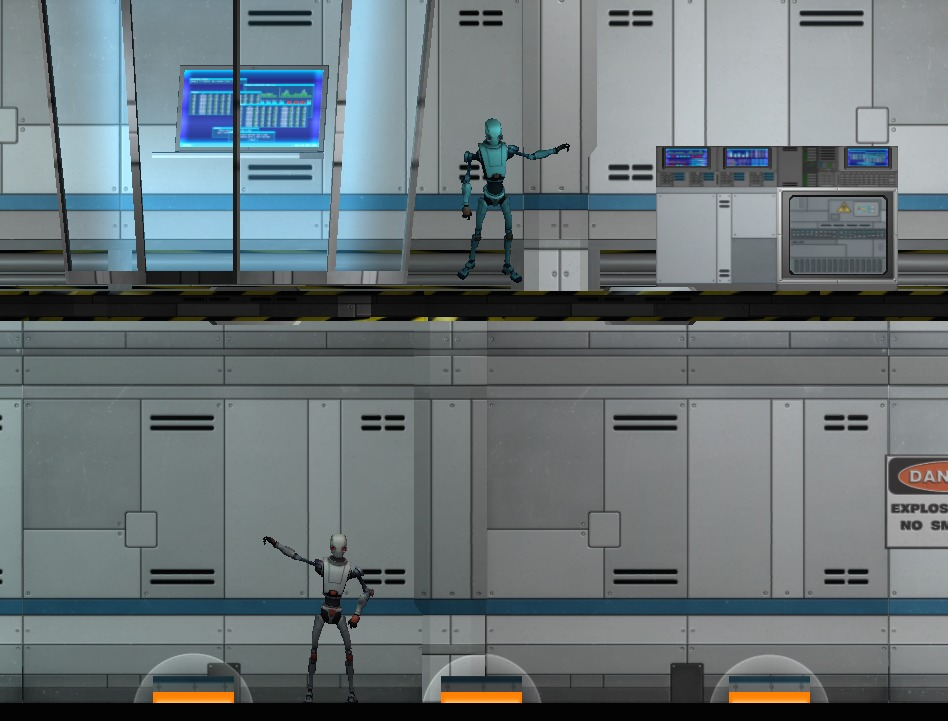
\includegraphics[width=0.7\columnwidth]{Figures/US_F2.jpg}
\caption{A sequence puzzle from Mute Robot. The top player knows the correct sequence and is showing the bottom player to move to and jump on the center yellow button among the three buttons.}
\label{fig:US_F2}
\end{figure}

\begin{figure}[!t]
\centering
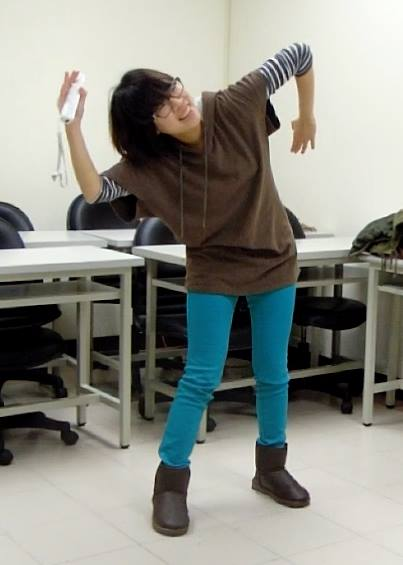
\includegraphics[width=0.4\columnwidth]{Figures/US_F3.jpg}
\caption{A participant performing a pictogram (the letter ``N'') using body language.}
\label{fig:US_F3}
\end{figure}


\subsection{Both Speaking and Body Language}
When both speaking and body language were available for communication, the players without common languages primarily used body language communication, and used tones and word to facilitate, such as when confirming a correct action. Players with common languages primarily communicated by speaking, and used body language to facilitate. 



\section{Player Feedback}
We summarize participants' feedback below:
\begin{enumerate}
  \item Fun: players reported that adding body language to cooperative gameplay enhanced gaming experience and enjoyment. For example, one participant reported ``body language is intuitive, without restriction, really funny and becoming an innovative way for a cooperative game.'' (P34), and another reported
	``For cooperative games, it's nice to be possible to be mis-understood, add something new to the gameplay'' (P18).

  \item Voice: players found that voice improved the gaming experience compared to only using body language. For example, one participant reported that ``it is too silent when playing with only body language, I feel less lonely with voice.'' (P5) and another said ``it is more fun to hear the other player in addition to body language'' (P19).


  \item Interactivity: players reported that having body language enriched the game's interactivity. For example, players reported ``Body language provides more challenges and feels like really playing with my partner.''(P37), ``I feel embarrassed talking to a stranger, but using body language is not.'' (P23), and another player reported ``It's great to move your body, and it's more interactive'' (P11). 


  \item Preferred communication methods: one player reported ``Using body language to communicate is more challenging, and more rewarding.''(P37), yet another player reported preference for having both speaking and body language because ``you can use whatever you prefer to communication to your partner to convey your meaning.''(P48). 

\end{enumerate}



\section{System Limitation}
Our prototype currently uses version 1 of the Kinect sensors, which can only track the major skeletal movements (head, torso, arms, and legs). It could not track more subtle expression such as eyes and facial expression, that are also important for non-verbal communication. In addition, it can not track finger and hand movement. As one participant reported: ``The avatar can't fully express what people can express, like emotional reaction.''

We plan to use improved sensors, such as the Kinect v2 sensors, that can capture players' more subtle movements such as hands and fingers. Furthermore, we plan to use computer vision techniques to capture and relay players' facial expressions.
